\documentclass [12pt,letterpaper]{report}

% Standard packages
\usepackage{amsmath}		% Extra math definitions
\usepackage{graphics}		% PostScript figures
\usepackage{setspace}		% 1.5 spacing
\usepackage{longtable}          % Tables spanning pages
\usepackage{verbatim}

% Vijay packages
\usepackage{url}
\usepackage{graphicx}
\usepackage[lofdepth,lotdepth]{subfig}

% Custom packages
\usepackage[first]{datestamp}	% Datestamp on first page of each chapter
\usepackage[fancyhdr]{McECEThesis}	% Thesis style
\usepackage{McGillLogo}		% McGill University crest

% $Id: ThesisEx.tex,v 1.1 2005/06/09 12:48:46 kabal Exp $

\usepackage{color}
\def\headrulehook{\color{red}}		% Color the header rule

%===== page layout
% Define the side margins for a right-side page
\insidemargin = 1.3in
\outsidemargin = 0.8in

% Above margin is space above the header
% Below margin is space below footer
\abovemargin = 1.1in
\belowmargin = 0.75in

%========= Document start

\begin {document}

%===== Title page

\title{A Tool for Configuring Mappings for Musical Systems using Wireless Sensor Networks}
\author{Vijay Rudraraju}
\date{\Month\ \number\year}
\organization{%
  \\[0.05in]
  \McGillCrest {!}{1in}\\	% McGill University crest
  \\[0.05in]
  Music Technology Area\\
  Schulich School of Music\\
  McGill University\\
  Montreal, Canada}
\note{%
  {\color{red} \hrule height 0.4ex}
  \vskip 2ex
  A thesis submitted to McGill University in partial fulfillment of the
  requirements for the degree of Master of Arts.
  \vskip 2ex
  \copyright\ \the\year\ Vijay Rudraraju
}

\maketitle

%===== Justification, spacing for the main text
\raggedbottom
\onehalfspacing
\pagenumbering{roman}

%===== Abstract, Sommaire & Acknowledgments
\section*{\centering Abstract}

Digital musical instruments, which are defined here as interactive musical systems containing a control mechanism and a sound generation mechanism, are powerful tools for analyzing performance practice and for transforming and reimagining the bounds of musical performance. However, the transitory nature of digital technology and the complexity of maintaining and configuring a digital musical instrument involving tens, if not hundreds, of interconnected, discrete components presents a unique problem. 

Even the most mechanically complex acoustic musical instruments, like a piano, are robust enough to withstand the daily grind without expert intervention by someone with intimate knowledge of the material and mechanical construction of the instrument. Furthermore, they are standardized enough that repairs can be conducted by any number of trained professionals. By contrast, digital musical instruments are often configured differently for each performance (this configurability being one of the virtues of a digital musical instrument), incorporate any number of non-standard pieces of hardware and software, and often can only be reliably configured by their creator.

This problem is exacerbated as the number of sensors that make up the control mechanism in an instrument increases and the interaction of the control mechanism with the sound generation mechanism grows more complex. This relationship between the control mechanism and the sound generation mechanism is referred to here as the "mapping" of the instrument. The mapping for an instrument represents the aspect of an instrument that is usually most configurable because it is defined by software (as opposed to hardware) and also most crucial to the character of the instrument. In the case of a digital musical instrument, being able to easily configure the musical instrument becomes a point of artistic freedom in addition to a point of maintainability.

This thesis builds upon work encompassed in two projects at the Input Devices and Musical Interaction Lab, the Digital Orchestra Project and libmapper, to tackle the problem of building an interface/system for configuring a complex musical system without expert programming skills. The intent is to present a targeted survey of user interface design and data visualization design research through the years to inform the design of a graphical user interface for performing this configuration task.

\newpage

\section*{\centering Acknowledgments}

Thesis regulations require that contributions by others in the collection of
 materials and data, the design and construction of apparatus, the performance
 of experiments, the analysis of data, and the preparation of the thesis be
 acknowledged.

%========== Tables of contents, figures, tables
\tableofcontents
\listoffigures
\listoftables

\newpage
\chapter*{List of Acronyms}\markright{List of Terms}

\begin{longtable}{ll}
  HCI		&	Human-Computer Interaction\\
  UID		&	User Interface Design\\
  DMI		&	Digital Musical Instrument\\
  EMI		&	Electronic Musical Instrument\\
  OSC	&	Open Sound Control\\
  IDMIL	&	Input Devices and Music Interaction Laboratory\\
\end{longtable}

\cleardoublepage
\pagenumbering{arabic}

%========== Chapters
\typeout{}
\resetdatestamp

\chapter{Introduction}

\begin{quote}
``Most principles of design should be greeted with some skepticism, for word authority can dominate our vision, and we may come to see only through the lenses of word authority rather than with our own eyes.

What is to be sought in designs for the display of information is the clear portrayal of complexity. Not the complication of the simple; rather the task of the designer is to give visual access to the subtle and the difficult - that is,

the revelation of the complex." - Edward R. Tufte, 2001 \cite{tuft2001}
\end{quote}

\section{Project Overview}

The goal of this research project is to apply a thorough understanding of a specific problem and a selection of theoretical principles in the areas of user interface design, data visualization, and human cognition to design a user interface that allows a user to solve this problem as effectively as possible. The problem addressed here is creating a mapping between a large number of signal sources and destinations distributed over many devices on a network to be used in a musical scenario. 

This research is an offshoot of a branch of research that began with the McGill Digital Orchestra Project \cite{orchestra2010}. The spirit and intent of the Digital Orchestra Project is understood as follows.

\begin{quote}
``Although designers of Digital Musical Instruments (DMI) are interested in creating useful, flexible, and creatively-inspiring interfaces and sounds, this process often depends on the vision and insight of a single individual. The McGill Digital Orchestra project instead brings together research-creators and researchers in performance, composition and music technology to work collaboratively in creating tools for live performance with digital technology." \cite{Malloch2007}
\end{quote}

The research project described in this thesis is a rethink of one particular aspect of the Digital Orchestra Project that is especially important.

\begin{quote}
``In the process of creating instruments for this project, we have found ourselves faced with the unique challenge of mapping new instruments in collaboration with experienced performers, as well as with composers tasked with writing pieces for these instruments. Because this ambitious project has taken on these three main challenges of the digital performance medium simultaneously, we have found ourselves in need of tools to help optimize the process. Specifically, mapping the various streams of controller output to the input parameters of synthesis engines has presented us with situations where both ease of use and flexibility were both [sic] of the utmost importance. We needed to be able to modify connections between data streams during precious engineer-composer-performer meeting time, while minimizing wasted minutes "reprogramming" our signal processing routines." \cite{Malloch2007}
\end{quote}

\begin{figure}[htb]
\centering
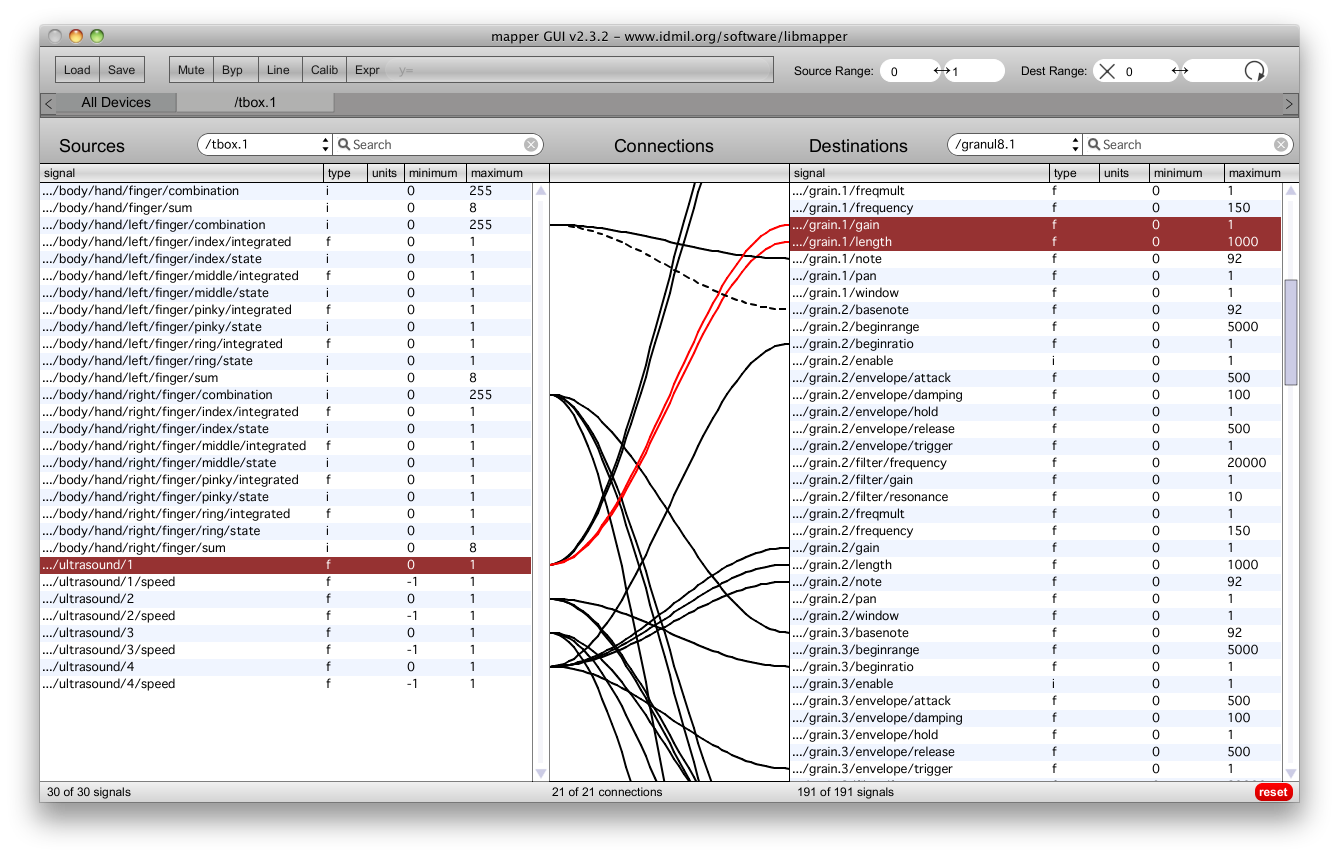
\includegraphics[width=1.0\textwidth]{maxmapper.png}
\caption{The Maxmapper GUI}
\label{fig:maxmapper}
\end{figure}

This portion of the Digital Orchestra Project is now referred to, at the Input Devices and Music Interaction Laboratory (IDMIL) at McGill University, as the \emph{Mapping Tools} project and includes the \emph{Digital Orchestra Toolbox} developed during the Digital Orchestra Project. The current manifestation of this research into simplifying DMI mapping is \emph{Libmapper}, a C library that implements the \emph{Mapper protocol} that is used to create mappings and the \emph{Maxmapper} graphical user interface (GUI) that is used to interface with the functionality that Libmapper provides. This GUI is called Maxmapper because it is implemented using the Max/MSP development environment and to differentiate it from \emph{Vizmapper}, the name of the alternative GUI developed through the research presented in this thesis.

The Maxmapper has been used by many musicians and composers and has proven its ability to simplify the DMI mapping task for non-programmers. However, the interface is typically used in situations where there are a small number of DMIs each with a small number of signals. Examining the interface in Figure \ref{fig:maxmapper}, it is clear that in a scenario with an order of magnitude more signals, the way that the data is \emph{visualized} will cease to provide the user with any understanding about the relational structure of a Mapper network or what configuration to use for a large network. Since the primary utility of a computer (in the sense of a being something that performs computations) is dealing with large bases of data and operating large numbers of things, this is a significant shortcoming of the user interface. After all, people performed computations before computers! We use computers because they can perform operations faster and in larger quantities than a human.

Computer systems engineers often talk about the ability of a system to \emph{scale}, meaning the ability of a system to gracefully handle an increasing number of users, machines, data stores, etc. without significant structural modifications or loss of utility. In some sense, what is happening is that the user interface and data visualization of Maxmapper does not \emph{scale} from DMIs to a larger sensor network.  The hope is that the research in this thesis contributes some insights into alleviating this interface problem and produces a successful alternative interface for configuring Mapper-based musical sensor networks.

\section{Thesis Structure}

This thesis is structured as follows:

Chapter 2 introduces the concept of mapping by providing a theoretical grounding of the concept as understood in mathematics and computer science and explains the more targeted concept of mappings in DMIs.

Chapter 3 examines the history of computer user interfaces as context for understanding a few principles discovered in the disciplines of user interface design, data visualization design, and cognitive science.

Chapter 4 uses these principles to design and implement a user interface for configuring mappings.

Chapter 5 concludes the thesis and presents hopes for future work on this topic.


%==========
\typeout{}
\resetdatestamp

\newcommand\Dfrac[2]{\frac{\displaystyle #1}{\displaystyle #2}}
\newcommand{\mathBF}[1]{\mbox{\boldmath $#1$}}
\newcommand{\C}[1]{\mathBF{#1}}

\chapter{Mapping}

\section{Mappings in Theory}

The term \emph{mapping} is used in mathematics, computer science, and related technical fields to encapsulate the concept of a \emph{function} and other related concepts under one abstraction. Like most technical terms used in multiple technical disciplines, the meaning of \emph{mapping} varies according to the context of the field that it is used. However in the case of mapping, the variation is subtle enough that a cursory understanding of the way mapping is used in a couple of contexts outside of DMIs might illuminate why it is a necessary and valuable concept to encapsulate in the context of new musical interfaces and help understand what is required for an interface designed specifically for mapping.

\subsection{Mappings in Mathematics}
\label{sec:Mappings in Mathematics}

In the mathematics context, the use of the term \emph{mapping} varies subtly according to the subdiscipline within mathematics in which it is used and often between specific mathematicians; however it is acceptable to use the word as a synonym for \emph{function}. A function in mathematics describes an associative relationship between two sets of numbers. One set of numbers is referred to as a \emph{domain} or \emph{set of inputs} and the other set is referred to as a \emph{codomain}, \emph{range}, or \emph{set of outputs}. Mathematicians often say that a function "maps" a domain to or onto a range, hence the reason for using the term \emph{mapping} as a synonym for \emph{function} \cite{functionMapping}.

To avoid confusion in later chapters, note that this the opposite of how outputs and inputs are referred to in a DMI mapping. The set of output signals is actually the domain of a DMI mapping and the set of input signals is the codomain of a DMI mapping. 

Strictly speaking in mathematics, a function can only represent a \emph{one-to-one mapping} or a \emph{many-to-one mapping}. It is helpful to know that a property of both types of mapping is that every element in the input (domain) set is associated by the function with one and only one element in the output (range) set. A corollary statement about both one-to-one and many-to-one mappings is that every element in the output set might be associated to one element (one-to-one) or many elements (many-to-one) in the input set. This language should become more clear as the usage of the terms \emph{one-to-one} and \emph{many-to-one} are explored in the remainder of the chapter.

The following are examples of equations that represent functions:

\begin{equation} \label{eq1}
y = f(x) = x + 1
\end{equation}
\begin{equation} \label{eq2}
z = g(x) = x^{2}
\end{equation}

In addition to both being functions, equation \ref{eq1} is a one-to-one mapping and equation \ref{eq2} is a many-to-one mapping. Basic types of functions like equations \ref{eq1} and \ref{eq2} often use the set of all real numbers (roughly, defined as any number that can be expressed as a potentially infinite string of digits - in the case of irrational numbers like \begin{math}\pi\end{math} - in decimal notation) as both the input set and the output set. Since the set of all real numbers is infinitely large, the association from one input element to one output element is described by a mathematical transformation that when applied to any element of the input set (the set of all real numbers) produces the element of the output set (the set of all real numbers) that the input element is mapped to. This is convenient because that means the function can be written very concisely in one line as opposed to two infinitely long columns with lines drawn between elements that are mapped to each other (not very convenient). 

Equation \ref{eq1} is the canonical notation for representing a mapping/function labeled \begin{math}f\end{math} where the input element is labeled \begin{math}x\end{math} and the output element is labeled \begin{math}y\end{math}. Equation \ref{eq2} represents a mapping/function labeled \begin{math}g\end{math} where the input element is labeled \begin{math}x\end{math} and the output element is labeled \begin{math}z\end{math}. 

To calculate the mapping that is implied by these two mathematical transformations, substitute any real number (since the set of all real numbers is the input set) for the symbol \begin{math}x\end{math}. By this logic, equation \ref{eq1} represents the mapping where every real number \begin{math}x\end{math} is mapped to the real number \begin{math}y\end{math} that is the value of \begin{math}x + 1\end{math}. Equation \ref{eq2} represents the mapping where every real number \begin{math}x\end{math} is mapped to the real number \begin{math}z\end{math} that is the value of \begin{math}x^{2}\end{math}. Equation \ref{eq2} is a many-to-one mapping because it maps both the positive and negative of every input number to the square of that number (the square of any real number is always positive), unlike equation \ref{eq1} which maps every input number to an output number that no other input number is mapped to.

\subsection{Cardinality in Mathematics}

There is more to be said about the concept of a one-to-one mapping and two related concepts, one-to-many mappings and many-to-one mappings. The framework for discussing different types of mappings is provided in one form by the mathematical concept of \emph{cardinality}.

First, three additional concepts should be enumerated and elaborated upon. These concepts are \emph{injection}, \emph{surjection}, and \emph{bijection}.

An \emph{injection} is a function that meets the condition that every element of the function's codomain (output) set is associated to no more than one element in the functions domain (input) set. Here, domain and codomain are used in the same way as in section \ref{sec:Mappings in Mathematics}.

A \emph{surjection} is a function that meets the condition that every element in the codomain set is associated to at least one element in the domain set.

A \emph{bijection} is a function that is both an \emph{injection} and a \emph{surjection}.

\begin{figure}[ht]
\centering
\subfloat[Non-injective and non-surjective][Non-injective and non-surjective]{

\includegraphics[width=0.35\textwidth]{200px-Total_function.png}
\label{fig:figure1}}
\qquad
\subfloat[Injection][Injection]{

\includegraphics[width=0.35\textwidth]{200px-Injection.png}
\label{fig:figure2}}
\qquad
\subfloat[Surjection][Surjection]{

\includegraphics[width=0.35\textwidth]{200px-Surjection.png}
\label{fig:figure3}}
\qquad
\subfloat[Bijection][Bijection]{

\includegraphics[width=0.35\textwidth]{200px-Bijection.png}
\label{fig:figure4}}
\caption{Four types of functions}
\label{fig:globfig}
\end{figure}

Figure \ref{fig:globfig} summarizes the possible types of functions using these distinctions.

Within mathematics, cardinality is a concept that allows one to reason about the relative sizes of different sets. It is particularly useful when comparing infinite sets. It allows one to reason correctly, for example, that the infinite size of the set of all real numbers is larger than the infinite size of the set of all positive integers (natural numbers). Yes, infinity can be proven to be larger than infinity!

Two sets are defined to have the same \emph{cardinality} if there exists a bijection between the two sets. It follows from the definition of injection that if there exists an injection from set \emph{A} to set \emph{B}, but no bijection, then the cardinality of B is greater than the cardinality of A \cite{cardmath2010}.

As mentioned before, these mathematical concepts are useful for describing one-to-one mappings and many-to-one mappings. In this terminology, injections and bijections are one-to-one mappings, whereas surjections and functions that are neither injections or surjections are many-to-one mappings.

\subsection{Mappings in Computer Science}
\label{sec:Mappings in Computer Science}

In the computer science context, a mapping is an abstract data type or concrete data structure, commonly referred to as an \emph{associative array} or \emph{dictionary} \cite{assocarray2008}.  

Abstractly and simply, the one and only way to store data of any kind (the value "0", the value "1", some text, an image, a sound, a recorded signal) in a computer of any kind, such that one can reliably retrieve the data later, is to put the data in some "bucket" that has some "label". The words "bucket" and "label", as used here, are not well-defined in computer science. But they help to unobtrusively make the point that if the data has no label that is associated with it or equivalently if the label has no unique memory location associated with it, then practically, it cannot be retrieved. In the scenario of a computer processor accessing internal memory, \emph{bucket} and \emph{label} could be replaced by \emph{memory location} and \emph{memory address} respectively.

As an example from the music information retrieval context, if a librarian wants to be able to store a large amount of sheet music such that it can be found later, the librarian needs some system to catalog or index the material such that a piece of sheet music can be referred to by some label. In the case of a library, this label is often a call number, the title of the piece, the name of the composer, etc.

Just like a reference library can use many different labeling systems to catalog the sheet music stored within its walls so that it can be retrieved with minimum headaches, a computer system can internally utilize many different abstract data types or concrete data structures. In both cases, the best choice is dependent on the material or data being cataloged or indexed. A mapping as a data structure in computer science parlance then, can be understood as a particular type of system for labeling data.

In particular, a mapping is a labeling system that is composed of a set of labels (keys) and a set of pieces of data (values), where every label in the first set is associated with one or many of the pieces of data in the second set. Then this structure encompassing the two sets and the list of associations between the two sets is given a higher level label that refers to the mapping as a whole. This allows one to construct a mapping of mappings, which lends itself nicely to hierarchical labeling systems.

This reframing of the term in the computer science context, as opposed to the mathematical context, focuses on one implication of the concept of mapping. One can specify multiple, unique mappings that each operate on the same collection of labels and the same collection of pieces of data. Similarly, one can specify multiple, unique functions that each operate on the same input set and the same output set. 

So in a computer system, one can create multiple mappings that each associate the same set of labels with the same set of data differently. This characteristic of mappings is one of the primary reasons why mappings are a useful frame for understanding the potential of digital musical instruments. 

\subsection{Cardinality in Computer Science}

Within computer science, cardinality is a concept used in relational database systems \cite{carddata1987}. 

A relational database can be seen as a very robust and flexible \emph{data labeling system}, in reference to the discussion in Section \ref{sec:Mappings in Computer Science}. A relational database is defined as a set of relations, where a relation is defined as a set of lists of attributes. Each list in the set has the same attributes as every other list in the set. An attribute defines a property that can take any value constrained by the set of values that are defined for each particular attribute. A relation is usually described by a table as in Tables \ref{tab:studentrelation}, \ref{tab:facultyrelation}, and \ref{tab:relation}. Together these three relations define one database.

\begin{table}
    \begin{center}
    \begin{tabular}{ | l | l | l | l | }
    \hline
    Student ID : Integer & Name : String & Thesis Topic : String \\ \hline
    00001 & Alice & 4d Maps \\ \hline
    00002 & Bob &  Anti-Gravity Toaster \\ \hline
    00003 & Carl & Invisible Clothing \\ \hline
    00004 & Doug & Personal Babel Fish \\
    \hline
    \end{tabular}
    \end{center}
    \caption{Example of a database defined by 3 relations - Student Relation}
    \label{tab:studentrelation}
\end{table}

\begin{table}
    \begin{center}
    \begin{tabular}{ | l | l | }
    \hline
    Faculty ID : Integer & Name : String \\ \hline
    0001 & Ohyes Hedid \\ \hline
    0002 & Ohno Hedidnt \\
    \hline
    \end{tabular}
    \end{center}
    \caption{Faculty Relation}
    \label{tab:facultyrelation}
\end{table}

\begin{table}
    \begin{center}
    \begin{tabular}{ | l | l | l | }
    \hline
    Pairing ID : Integer & Faculty ID : Integer & Student ID : Integer \\ \hline
    00000001 & 0001 & 00004 \\ \hline
    00000002 & 0002 & 00002 \\ \hline
    00000003 & 0001 & 00003 \\ \hline
    00000004 & 0001 & 00001 \\ 
    \hline
    \end{tabular}
    \end{center}
    \caption{Pairing Relation}
    \label{tab:relation}
\end{table}

In a relational database, the cardinality of an attribute is the number of instances of that attribute that can be associated with a given set of instances for other attributes. In a database as in DMI mapping, it is largely sufficient to distinguish between a cardinality of \emph{one} and a cardinality of \emph{many}.

The simple database composed of the relations in Tables \ref{tab:studentrelation}, \ref{tab:facultyrelation}, and \ref{tab:relation} provides an example to reason about the cardinality of database relations. If every student (represented by their ID) has one advisor (also represented by their ID) but every advisor has many students, then the relation is one-to-many from Advisor ID to Student ID. Since the horizontal ordering of attributes has no meaning in a relation, we can also reason that the relation from Student ID to Advisor ID is the reverse, many-to-one. Finally, every student has one thesis topic and each thesis topic is the topic of one student so the relation is one-to-one from Student ID to Thesis Topic.

These mathematical and computer science concepts provide a solid foundation for understanding the various nuances of mapping abstractly and concretely. This background will be necessary to create a well-informed user interface for creating and modifying DMI mappings.

\section{Mappings in Digital Musical Instruments}
\label{sec:Importance of Mapping}

In an acoustic musical instrument, the equivalents of the "control mechanism" and "sound generation mechanism", as they are called in a DMI, are \emph{intrinsically coupled} or bound to each other because the physical material (e.g. wood, metal, horse hair) of the instrument that forms the control mechanism also forms the sound generation mechanism. Making a decision that alters the control mechanism will significantly or subtly alter the sound generation mechanism. Replacing the horse hair of a violin bow with artificial fiber will result in a perceived difference in tone to the trained ear.

In a DMI, the control mechanism is composed of sensors typically embedded in structural materials that form the shape of the instrument and connected to a microcontroller that provides the interface for accessing the sensor signals. The physical gestures of the performer are not coupled to the sound generation through purely mechanical means, but through electrical means. Each sensor, whether it senses acceleration, orientation, touch, etc. produces an electrical signal that correlates to some physical measurement. This analog electrical signal is converted to a digital signal through some kind of analog to digital signal conversion (perhaps within the control mechanism on an integrated microcontroller) and then this digital signal is processed by a computer and sent to the sound generation mechanism, which is a piece of software that produces audio samples.

The following illustrative example makes clear that the control mechanism and sound generation mechanism are not \emph{intrinsically coupled} in a DMI as they are in an acoustic musical instrument.

If one takes a control mechanism with embedded touch sensors, records an output signal produced by a performer with the control mechanism on a hypothetical signal recorder, and replaces the connection between the control mechanism and the sound generation mechanism with a connection between the signal recorder and the sound generation mechanism, it is clear that the active control mechanism of the DMI has changed. The control mechanism is now the signal recorder. The original control mechanism with the touch sensors is no longer part of the DMI system because it is disconnected from the DMI. But this change results in no change within the sound generation mechanism. The sound is generated by software that produces audio samples and thus is not affected by a change to the physical hardware of the control mechanism as long as the control mechanism produces an output signal that is identical. If the performer presses play on the recorder it will be impossible to tell the difference between the initial DMI and the modified DMI purely from the sound generated by the DMI.

In physical terms, when two formerly intrinsically coupled aspects of system are free to become uncoupled, a new degree of freedom is introduced. One imprecise way to understand why this happens is that the "signal" (used loosely) controlling the sound generation is no longer all the vibrations in the physical body of the instrument (in an acoustic musical instrument), but a discrete electrical signal that travels through a very specific electrical channel (in a DMI).

In the context of DMI research this new degree of freedom is the freedom to choose a mapping \cite{hunt2003}. Mapping as used in this context is very similar to how the term is used in both the mathematics and computer science context. Each context provides an understanding that is well suited to manipulate one of two possible conceptual layers in a mapping system. These two contexts have also been referred to as a \emph{systems} point of view and a \emph{functional} point of view respectively \cite{nort2010}. 

\begin{enumerate}
\item The set of sensors embedded in the control mechanism outputs a set of signals, which we will refer to as \emph{output signals}. The sound generation mechanism outputs sound that is controlled through a set of \emph{input signals} defined by the software that is responsible for the sound generation. Therefore, for any given control mechanism and sound generation mechanism there is a choice of how to associate the two sets of signals (output signals from the control mechanism and input signals from the sound generation mechanism) with each other, much like an associative array in the computer science context. Importantly, this is a choice that is not independently available when constructing, for example, a violin because the two sets of signals (if this distinction between control mechanism and sound generation mechanism is imagined in a violin) in a violin are physically coupled and inseparable. It is not a choice that is explicitly made when constructing an acoustic instrument.

\item Furthermore, there is a second, lower level form of mapping when dealing with a specific pair of associated signals. Because it is unlikely that any given signal output by a control device is calibrated to a particular input signal in a sound generation device that one might associate with the given output signal, we require a second set of relations beyond a binary associated/not associated. Any given output signal might be capable of outputting values that are outside the set of values that a particular input handles or simply be outputting a different data type altogether. In electronics, this is called \emph{signal conditioning} and can be handled completely in the analog components that produce the signals. If this signal conditioning is not handled in the analog hardware and is modified dynamically in the software of the DMI, after analog to digital conversion of the signal, then this signal conditioning is handled by the mapping system. In this case, a mapping in the functional, mathematical sense of the word is necessary to transform the output signal so that the values reliably fall within the set of acceptable input values. Performing signal conditioning as part of the DMI mapping, as opposed to as part of the control mechanism, has the benefit of not requiring any change in the analog electronics of the DMI, if the associative mapping layer changes.
\end{enumerate}

A prototypical mapping system can specify not only the associations between two sets of signals (pairs of connected signals), but associate a function with each pair of connected signals that specifies how to transform/condition the signal before copying the value to an input. This function might, in fact, be simply \begin{math}y = x\end{math} in the case where no calibration is needed, however the point is that it is not practical to assume that this will always be an acceptable mapping function between an output and input. Therefore, signal conditioning might be useful to include as a second layer in a mapping system.

This physical decoupling between the control mechanism, the mapping system, and the sound generation mechanism creates a modularity between the three components that can be exploited to simplify the DMI development and maintenance process.

\section{A Dedicated Mapping System: Libmapper}

The creation, evolution, and stabilization of the design of a DMI is inherently a tightly iterative process. A violin luthier must be comfortable enough playing a violin to develop an aesthetic sense of what effect the countless decisions that are made in the process of building a violin have on the experiential quality of the instrument that they are creating. Whether a particular decision is the right one can only truly be evaluated after the decision is made and someone plays the violin. 

Similarly, a team of people building a DMI will often make a construction decision, evaluate the effect of that decision, make some changes, and repeat. This process is often referred to as \emph{iterative development} and occurs in any serious design process whether or not it is ever made explicit \cite{iterative2003}. 

Because such iterative development is so beneficial to the development of DMIs, people often use various platforms and frameworks as common foundational building blocks for such systems. These environments often take care of implementing higher level functionality for controlling and generating audio in realtime or interfacing with hardware. Thus, they allow one to quickly test ideas for a DMI and focus on experimenting with the aspects of the control mechanism and sound generation that are unique to the particular project before investing too much time and money into custom parts without assurance that the ideas are viable in a basic sense. For the control hardware, there are platforms like Arduino. Coding environments like Max/MSP and code libraries like STK simplify the development of synthesizer modules for sound generation. In an effort to provide a similar foundation for creating mapping systems, the Digital Orchestra Toolbox was created as part of the McGill Digital Orchestra project and includes components representing the common subroutines used in a mapping system. More recently, this functionality has been reimplemented as a C library called Libmapper at IDMIL, a lab at McGill University. Libmapper has several characteristics which make it a desirable system for configuring mappings. 

One is that a mapping between control and sound generation can be modified without recompiling any code, restarting any system, or reloading any script. Typically, if a mapping is specified in software through a Max/MSP program, C program, etc. then the part of the code that specifies the mapping must be modified and recompiled or reinterpreted before the new mapping becomes active. Any DMI that embeds Libmapper in its control and sound generation software can have its mapping modified simply by being sent specific messages as specified by the mapping protocol. 

Another useful characteristic is that, in the case of a local network with many different control mechanisms and sound generation mechanisms available, no central device is needed to facilitate communication between devices. If one component on the network experiences some difficulties, the other devices will still be able to keep the mappings between the remaining devices operating.  

Lastly, and of particular relevance to the primary topic of this paper, is that the current state of mappings between various devices on the network can be viewed and modified by any graphical user interface that embeds Libmapper. In Libmapper parlance, these applications can register as \emph{monitors}. Because of this capability, multiple members of a team can be viewing and modifying the same mappings for multiple DMIs using different computers and using different graphical user interfaces.  

A network with Libmapper-enabled devices and monitors is a \emph{Mapper network}.

\subsection{Open Sound Control Protocol}

Seen from a bird's eye conceptual level, Libmapper is an implementation of a communication protocol that was created for specifying mappings over a distributed network \cite{Malloch2009}. 

A communications protocol is a rigorous and formal description of a message format and rules for exchanging messages adhering to the protocol. The term ``protocol'' usually refers to the formal description of the protocol and is distinct from the implementation of the protocol. A protocol without an implementation is analogically like a constitution without a government. If two devices adhere to the same protocol then they are able to reliably communicate with each other because they can, in a sense, speak the same language. The Mapper protocol is itself defined in terms of the Open Sound Control (OSC) protocol. This is a common practice for constructing increasingly specific protocols. The Internet is essentially a particular stack of protocols that are layered on top of each other and specify how devices and routers are to be addressed, open connections with each other, and interpret messages.

To say that one protocol is layered on top of another is to say that the higher level protocol is defined in terms of the structure and conventions of the lower level protocol. In the case of Libmapper, the protocol layer that the OSC protocol is implemented on top of is called the User Datagram Protocol (UDP). The other common protocol that can be used at this conceptual layer of the Internet protocol stack is the Transmission Control Protocol (TCP). The well-known Hypertext Transfer Protocol (HTTP) is layered on top of TCP. A web browser implements HTTP so that it can fetch and display web pages from remote systems that speak the same protocol. As a protocol, OSC in not defined in terms of a particular Transport protocol (the name given to the layer in the protocol that UDP and TCP occupy - HTTP occupies the layer on top of the Transport layer, known as the Application layer). This is different from HTTP, which is specifically a TCP-based protocol.

Libmapper then allows one to configure a mapping relationship between any collection of devices (control devices, sound generation devices, and anything else) by embedding Libmapper into the code for each device and creating an instance of Libmapper upon startup of each device, thus allowing any system on a local network to easily implement the Mapper protocol without in-depth knowledge of the protocol.

The specification of the OSC protocol can be found on the web \cite{osc2011}. In the opinion of the creators of the protocol \cite{osc2009}, OSC is a "weak" form of protocol because it does not define certain necessary aspects of any form of data transmission. It does not define the patterns of command and response, error handling or receipt acknowledgement - only the format of the messages that are sent. These aspects are left as decisions to be made by particular implementations of the protocol or a protocol stacked on top of OSC.

The complete definition of the OSC protocol is not important for the scope of this thesis, however the following aspects of the protocol should give a sufficient sense of what is defined:

\begin{description}
\item a unit of transmission is a \emph{OSC Packet}, which consists of a contiguous block of binary data that is the contents of the packet and a number reflecting the number of bytes of data in the contents
\item the size of an \emph{OSC Packet} is always a multiple of 4 bytes
\item the contents of an \emph{OSC Packet} is an \emph{OSC Message}
\item an \emph{OSC Message} consists of an \emph{OSC Address Pattern} followed by an \emph{OSC Type Tag String} followed by zero or more \emph{OSC Arguments}
\item an \emph{OSC Address Pattern} is a URL-like string strictly beginning with the '/' character
\item an \emph{OSC Type Tag String} is a string strictly beginning with the ',' character followed a number of characters corresponding to the number of \emph{OSC Arguments} each of which specifies the OSC defined data type of each argument
\end{description}

\subsection{Mapper Protocol}

The semantics for the common set of OSC messages that the \emph{Mapper protocol} (the name that will be used to describe the specification implemented by Libmapper in this paper) is intended to be as useful as possible for configuring mappings between output and input signals without assuming too much about what form the control or sound generation will take. In the Mapper protocol, there is a concept of \emph{source device} and \emph{destination device}. In a DMI, the control mechanism will often be announced as a source device and the sound generation mechanism will be announced as a destination device. 

The set of messages proposed by the Mapper protocol allows each device participating in the composite distributed system to \emph{announce} its presence, \emph{discover}, \emph{describe} itself, \emph{link} to another device, \emph{connect} one of its signals (also referred to as datastreams) to a signal on a device it is linked to, and \emph{condition or transform} a signal with a basic mathematical function \cite{Malloch2009}. These last two pieces of functionality are the two possible levels of mapping that can be present in the prototypical mapping system referenced in Section \ref{sec:Importance of Mapping}.

The messages that are used to perform specific operations on the network have their own Mapper syntax distinct from OSC syntax. This syntax is used to improve readability and is transparently translated into OSC syntax by individual Libmapper instances before transmission over the network.

\subsubsection{Announcement}

Each device in the distributed system announces itself with a port and unique name that it would like to be addressed by. In the case that other devices on the local network have already reserved a particular port or unique name, Libmapper uses a collision detection algorithm to systematically try other ports and/or modify the requested name with an appended unique ordinal number. This allows a set of identical control or sound generation devices to each be programmed to request the same collection of OSC names for their signals without worrying about the identical devices being addressed by the same names.

The device is also responsible for declaring the signals that can send as output or receive as input. These signals are addressed by hierarchical OSC Address Patterns with the device name that the signal is associated with as the root of the address pattern. Therefore a device named \verb#tstick# with an assigned ordinal of \verb#2# would be addressed as \verb#/tstick.2# and an accelerometer signal on the device could be addressed as \verb#/tstick.2/accel/1/x#. A second signal might be addressed as \verb#/tstick.2/accel/1/y# and a third signal, \verb#/tstick.2/accel/2/x#. The fact that the name of every signal is formatted as a hierarchical namespace will be useful when deciding on the best visualization for this data.

\subsubsection{Discovery}

After a device appears on the network, announces itself, and receives a unique name and port number on the local network through the port and name allocation algorithm, it sends the following message to request that all Libmapper-compatible devices describe themselves:

\begin{quote}
\verb#/who#
\end{quote}

Other devices are obliged by the protocol to respond with (for example):

\begin{quote}
\verb#/registered /tstick.1 @inputs 1 @outputs 52 @class /tstick# 

\verb#  @IP 192.168.0.3 @port 8001#

\verb#/registered /granul8.1 @inputs 80 @outputs 0 @class /granul8#

\verb#  @IP 192.168.0.4 @port 8000#
\end{quote}

In this way any device or monitor (in the case of a graphical user interface) can request the names, IP addresses, and UDP ports of any devices on the network. 

\subsubsection{Device Linking}

To create a direct network link between two devices, the Mapper protocol specifies the following message:

\begin{quote}
\verb#/link /tstick.1 /granul8.1#
\end{quote}

Libmapper creates a router in software, which can be thought of as a special virtual device distinct from source devices and destination devices, for each pair of linked devices. In Mapper protocol terminology, a link is created between a source device and a destination device. Every router is tasked with the signal conditioning and message transformation for any pair of connected signals involving the two devices in the source/destination link pair that the specific router is created by Libmapper to manage. This Libmapper design decision allows each device acting as a source in a link to handle the traffic and processing of the links that it is involved in, thus distributing the work load over all source devices as opposed to assuming a single central router handling all traffic between all linked devices in the system.

When the Libmapper instance in the source device successfully creates a router for the link and completes initialization of the connection after receiving a \verb#/link# message, it responds with:

\begin{quote}
\verb#/linked /tstick.1 /granul8.1#
\end{quote}

Two devices are unlinked by sending the following message:

\begin{quote}
\verb#/unlink /tstick.1 /granul8.1#
\end{quote}

The source device then destroys the router handling this link after receiving a \verb#/unlink# message, and responds with:

\begin{quote}
\verb#/unlinked /tstick.1 /granul8.1#
\end{quote}

\subsubsection{Signal Connection}

Once a router has been created between a source and destination by requesting a link, specific output signals on the source device can be connected to specific input signals on the destination device. For example, once a T-Stick \cite{tstick2007} (\verb#/tstick.1#) has been linked to the Granul8 granular synthesizer (\verb#/granul8.1#), the individual signals output by the touch sensors, accelerometers, etc. in the T-Stick can be routed to specific inputs in the granular synthesizer. Without specifying connections between output signals and input signals, gestures performed with the control source device will have no affect on the audio samples produced by the sound generation destination device and the DMI will produce no sound. 

In the Mapper protocol, this is accomplished by sending a message similar to these:

\begin{quote}
\verb#/connect /tstick.1/raw/pressure /granul8.1/gain#

\verb#/connect /tstick.1/raw/pressure /granul8.1/gain#

\verb#  @scaling expression @expression x*10 @clipping minimum 0#
\end{quote}

The router managing the link between \verb#/tstick.1# and \verb#/granul8.1# records all the relevant information communicated by the \verb#/connect# message, sets up the address translation and transformation required to connect the output signal to its associated input signal, and responds with:

\begin{quote}
\verb#/connected /tstick.1/raw/pressure /granul8.1/gain#

\verb#/properties /tstick.1/raw/pressure /granul8.1/gain#

\verb#  @scaling expression#

\verb#/properties /tstick.1/raw/pressure /granul8.1/gain#

\verb#  @expression x*10#

\verb#/properties /tstick.1/raw/pressure /granul8.1/gain#

\verb#  @clipping minimum 0#
\end{quote}

A signal pair is disconnected by sending:

\begin{quote}
\verb#/disconnect /tstick.1/raw/pressure /granul8.1/gain#
\end{quote}

The router responds with:

\begin{quote}
\verb#/disconnected /tstick.1/raw/pressure /granul8.1/gain#
\end{quote}

The properties of a connection can be queried with:

\begin{quote}
\verb#/connection/properties/get /tstick.1/raw/pressure /granul8.1/gain#
\end{quote}

The syntax of the message for modifying properties of a connection is similar to creating a connection with \verb#/connect# replaced by \verb#/connection/modify#.

It may be noticed from this syntax that the Mapper protocol supports only \emph{one-to-one} and \emph{one-to-many} mappings between sets of signals. An output signal can be connected to one or many different input signals. However, the syntax does not provide a mechanism for specifying how to handle one input signal receiving a signal from multiple output signals. The added complexity of handling a \emph{many-to-one} or \emph{many-to-many} mapping maybe introduced into the Mapper protocol at a future time.

These special Mapper messages as defined by their message headers and syntax comprise what is referred to in this paper as the \emph{Mapper protocol}. By sending messages from this set of messages recognized by Libmapper it is possible to configure mappings between an arbritrarily large collection of devices on a local network with relatively little work and without understanding OSC.

\section{Sensor Networks}

A \emph{sensor network} is a term used in electrical engineering literature to refer to a system that employs a (typically) large number of distributed sensors that are connected to each other through autonomous, intermediary nodes capable of processing and communicating the data obtained from the particular sensors it is attached to and relaying that information to other nodes on the network. If the nodes communicate with each other through some form of wireless radio then the network can be referred to as a \emph{wireless sensor network}. The key functional difference being that in the wireless scenario, the nodes are not tethered to a particular physical location and are free to move provided they remain within radio range. Libmapper can, in principle, with few to no modifications operate in either scenario and the phrase \emph{sensor network} will be used to encapsulate both.

The concept of a sensor network is useful because it strikes a good balance of specificity and abstraction when describing a particular network topology and implementation. Sensor networks, particularly wireless sensor networks, are an active field of research in a diverse array of research fields including defense, environmental monitoring, energy/heat systems, and structural engineering. In these and related situations, the function of the sensor network is to sense, measure, and gather information from the environment and/or actors in the environment and use the capability of distributed processing nodes to make decisions about where the information should be routed \cite{survey2008}. The majority of research applications do not focus on the use of these datastreams to output sound, visuals, or control actuators in realtime, however the definition of a sensor network does not preclude the nodes in the network from being connected to actuators as well as sensors.

\section{Digital Musical Instruments as Localized Sensor Networks}

A DMI can be understood as a particular form of sensor network that is particularly localized and stable. Particularly, if all of the sensors, processing nodes (perhaps each running an instance of Libmapper), and sound generation mechanism are all housed in a single physical object. Typically, no academic would refer to such a DMI as a sensor network, however it would technically fall under the working definition used in this paper. A sensor network may include functionality that compensates for unreliable sensors and devices that enter and leave the network relatively often, especially for a large, distributed network, which is not necessary in a DMI with comparatively few and robust sensors. The larger the network, the more effort must be made to handle sensor and device failure. Hardware failure and reliability is a topic outside of the scope of this thesis, but is an important practical distinction between systems that are typically termed \emph{DMIs} and systems termed \emph{sensor networks}.

Framing a DMI as a sensor network affords one the ability to imagine what form a more \emph{sensor network-like} DMI might take. Additionally, because the task of mapping is fundamentally seen as a task of network topology configuration in this thesis, it is a better term to use when focusing on the mapping layer of a musical system. A single DMI might consist of many spatially-distributed control devices that each output signals connected to the inputs of a sound generation device. Or an orchestra of DMIs might be understood to be one musical sensor network that together produce one collection of sound. The argument is that understanding what is being built in terms of a sensor network, as opposed to individual DMIs that may or may not be played together, better reflects the pecularities of what a DMI fundamentally is and why the task of building a DMI is so different from building an acoustic musical instrument.

Additionally, perhaps such a reframing might better work \emph{with} the pecularities of a DMI and lessen the extent to which design teams work against the inate characteristics of computers attempting to make DMIs in the image of acoustic musical instruments. After all, as previously discussed, this fundemental difference between a DMI and acoustic musical instrument is what introduces the task of mapping as unique to DMIs in the first place. For convenience, the term \emph{musical sensor network} (MSN) will be used in the remainder of this paper to reference this particular framing of the DMI concept in contexts that might be helped by this alternative concept. However, the two terms can usually be used interchangably without being inaccurate. 

\section{Usability and Graphical User Interfaces}

Imagine a MSN comprised of more than ten Libmapper-enabled devices, some of them are control devices and some are sound generation devices. Each device might output, or receive as inputs, around ten signals. So to create a mapping layer over this distributed network of devices, one might send hundreds of Mapper protocol messages to link, unlink, connect, disconnect, etc. various pairs of devices and signals as one attempts to determine through trial and error the specific set of connections and functional transformations that best fit the particular sensors, devices, context, and design intentions of the people constructing the system. 

It may be that it is unclear what control device ought to be linked to what sound generation device, much less what signals within the control device to connect to what particular signals within the sound generation device. When experimenting with a mapping layer for a specific MSN it is necessary to view the current network mapping, modify the current mapping, test the new mapping, evaluate its effectiveness and then repeat the process until the mapping is satisfactory. 

Any tools and interfaces that speed up this iterative process and reduce the amount of Libmapper-specific/Mapper protocol knowledge required to efficiently explore the possibilities of a particular MSN improves the usability of Libmapper and allows for a wider diversity of skill sets and roles in a broader performance project involving instrumentalists, composers, directors, and engineers to participate in the mapping task that is so crucial to the character of a musical system. 

Advances in user interface design are, historically, a need driven by the specifics of the nature of the system that the user requires an interface to manipulate. Similarly, data visualization design is driven by the need of a user to develop understanding of a system from a complex set of data about the system so that they can correctly manipulate the system to match their intentions. 

This chapter has been a foundation for understanding the interface and visualization design decisions that are made in Chapter 4 as coupled to the requirements and need for a mapping system. The next chapter presents a foundation for understanding the decisions in Chapter 4 as coupled to what is known about what type of visualizations make a system easy to understand and what type of interfaces are effective for manipulating systems.


%==========
\typeout{}
\resetdatestamp

\chapter{User Interface and Data Visualization Design}

The bounds of the discipline of \emph{human-computer interaction} varies depending on who is asked. At present, people who practice the discipline understand human-computer interaction (HCI) to involve "the design, implementation and evaluation of interactive systems in the context of the user's task and work" \cite{hci1998}. 

Within the broad domain of interactive systems, different subdisciplines within human-computer interaction (HCI) focus on different aspects of the systems. Designing a user interface for manipulating a Mapper network is an interesting task because the design problem is a composite of two interrelated subproblems. The first is visualizing the current state of the Mapper network in such a way as to allow a user to quickly reason about the current state of the network. Solving this first problem effectively helps with the second problem, which is creating an interface that allows a user to determine what actions within the interface should be taken to move the network to a different, more desirable state. 

Conveniently there are two subdisciplines within HCI that task themselves with analyzing precisely these two problems: \emph{user interface design} and \emph{data visualization design}. Literature in these fields have much to say on the topic of how to proceed with the design of an interface and this chapter will focus on the findings that are most relevant to Vizmapper. To better understand the broader context of HCI, this chapter begins with a history of user interfaces in relation to the parallel history of general purpose computers.

\section{Short History of User Interfaces}

The term \emph{user interface} is a byproduct of historical developments in computing and makes best sense in the context of modern computing culture. The use of \emph{user interface} as a distinct concept was not needed when the \emph{user} was certain to be a professional engineer or programmer involved in the creation of the program and/or the machine that was to run the program; at the very least, they were comfortable interacting with the computer using the same means as the original programmer and did not require an explicitly designed interface to augment the usability of the system \cite{continuity1990}. Since \emph{user} is such a vague term, \emph{computer interface} is often used to refer to the part of the system that is meant by the term \emph{user interface}. This part of the system is the computer's interface to the world - whether the \emph{user} is assumed to be a programmer, a musician, another machine, the larger environment, or a poodle. 

The concerns of user interface designers have changed considerably since people first started interacting with programmable digital computers for processing, storing, and retrieving information. Understanding the context of and nature of the interdependant effect that fundemental developments in computing and their accompanying user interfaces have on each other helps one appreciate the impact that a seemingly frivolous thing like user interface can have on the development of the basic functionality of the computer - for example, the function  of using a computer for creating mappings between a distributed network of devices.  

\subsection{Punch cards}

The oldest computer interfaces largely depend on punch cards and paper tape as control mechanisms and paper printers for output and program feedback. On machines used during the 1950s and 1960s, in order to input a program and a dataset into a computer, first one prepares a deck of punched cards with a typewriter-like machine, then one feeds the deck to the computer \cite{oshistory2011}. Some machines can also mount reels of magnetic tape that store oft-used or previously generated datasets or precompiled complimentary software. On these early machines, a particular program being run from a deck of punch cards is assumed to have control of all the available resources of the computer. There would be no other resident software running on the machine handling auxilery tasks like on modern computers. Any hardware devices required by a particular program like punch card readers and line printers had to be handled completely by the user program contained in the deck of cards fed to the machine. 

\emph{Operating systems} development grew out of the growing complexity of computer systems involving many cooperating devices, which themselves mirrored growth of the complexity of the programs that were written for them. It makes little sense for a user of a machine to write basic operating software for interfacing with the same perhipheral devices as every other user of the computer everytime they want to run a program on such a machine. Since any user of a computer during the 1960s needed to enter a queue to reserve time to run their program on a machine they shared with their entire organization, any time wasted debugging low-level interactions with input and output devices is a major setback. Consequently, machines were developed that included libraries of code to take care of low-level control and provide easier access to input and output devices as always resident services. This collection of software that is permenantly resident on a machine became known as a \emph{batch monitor} \cite{os2000}. A user's program could link to these preloaded libraries without including the operating logic explicitly within their own program code. This shift is often cited as the genesis of the modern operating system.

In addition to providing access to input/output devices, the monitor provides services to perform error checking on user submitted programs and for generating useful feedback to the user concerning the progress of execution of a user program. The idea of generating "useful" feedback, and what that might mean, can be understood as the first instance of an explicitly designed user interface and the birth of user interface design \cite{unix2008}.

\subsection{Command-line}

Command-line interfaces are the next step in the evolution of computer interfaces and the link between batch systems of the 1950s and what would be recognized as a \emph{graphical user interface} (GUI) today. As processors developed further and resulted in the reduction of the amount of time needed to execute a basic operation on data, it became possible to interact with the computer more granularly with a series of requests, execute programs more instantaneously, and receive responses expressed as specially formatted strings of text using a specialized vocabulary. Requests could be completed in seconds, no longer hours and days, and it made sense for the user to simply wait for the request to be completed before entering in the next request. This is as opposed to sequencing a stack of commands in the form of a batch request and waiting for all the commands to be completed or for one of the command to fail. Instead, the user can change their mind about the structure of commands in the composite program in response to feedback from earlier commands. This introduces the possibility for software to explore a set of possibilities with the guidance of the user and allows for a type of interactivity not possible with the batch systems of the 1950s. 

Although the earliest command-line systems borrow typewriter-like teletypes (as used for telegraph transmission) as the input and output mechanisms, by the 1970s video display terminals are used with computers for providing text feedback on a virtual canvas of pixels that can be rapidly and reversibly modified (unlike teletype printers) and a program can display an interface that could be called visual as well as just textual \cite{unix2008}. This allows programmers to create the first computer games and text editors that rely on this capability of video display terminals.

\subsection{Graphical}

Further reduction of the amount of time a processor needed to execute individual operations results in the ability for the computer to communicate with multiple input/output devices in realtime. Typical devices that a modern computer program expects to have access to through the operating system include a color monitor wherein each pixel in the monitor had a separate referenceable address, a graphics card to help with processing of 2d/3d graphics operations, a mouse, a keyboard, and a sound card connected to audio speakers.

Much of the common grammar of all the popular graphical user interfaces in use today are derivatives of two particular projects. The first is called NLS/Augment (NLS stands for oN-Line System) and was designed by Douglas Engelbart and his team at the Stanford Research Institute. During a famous, public demonstration of the system in 1968 (often affectionately referred to as "The Mother of All Demos"), Engelbart proceeded to demonstrate the use of a computer mouse, a graphical display with multiple windows, and hyperlinks among many other notable advancements in human-computer interaction. 

The second groundbreaking project, the Xerox Alto, came from the Xerox Palo Alto Research Center (PARC) in 1973. It is perhaps the first computer designed from inception to be dedicated to the use of a single person, hence the introduciton of the term \emph{personal computer}. Although the monitor displays only black and white pixels, the graphical user interface of the operating system contains buttons, windows, scrollbars, sliders, and many of the logical GUI components that are standard components of any program with a GUI. It is followed at PARC by the Xerox Star in 1981, which takes GUIs a step further towards their current incarnations and introduces the ability to share resources across a local area network \cite{xeroxstar1989}.

It is primarily the ideas that these two projects consolidate and introduce to the wider world that eventually becomes the impetus for the recognition of HCI and, of more precise relevance to this paper, user interface design as important areas of study of significant relevance to the broader computer science community. 

\subsection{Five Foci of Interface Development}

It is clear from history that, in some sense, computing machines have always had user interfaces. What changes is the the level of attention that any particular layer in the computing interface receives during various periods of history. Grudin \cite{continuity1990} introduces a helpful framework for understanding this change that takes place during the second half of the 20th century as movement through five different foci of interface design. 

Initially, during and before the days of punch cards, most users of computers are electrical engineers primarily concerned with working directly with the hardware (flipping switches, replacing vacuum tubes, wiring ports and circuits). Conceptually, the computer interface is located at the hardware itself. 

Afterwards, the primitive operating systems and batch monitors place the majority of focus on the task of programming and the environment in which commands are executed and requests are made and begins shifting focus away from the hardware. The development of ever higher-level languages and environments eventually replaces the need to be familiar with hardware particulars. At this point, the primary interface in these systems is at the level of the software code and programming. 

As machines begin to perform their operations more quickly, systems become interactive and users are not expected to be able to interact with the computer through computer code, the interface grows into the canonical monitor, keyboard, and mouse of the 1990s and 2000s. It makes sense for designers of computer systems to become more concerned with issues of perception and motor control. 

In recent years it has become practical to interact with the computer in a more conversational/realtime manner and system designers focus on the entire process of a user interacting with the system over an extended period of time, from initial exposure to practiced expert interaction. The focus of the interface designer becomes less trained on issues of ergonomics and visual perception and more trained on deeper cognitive issues like learning and problem solving. The interface now encompasses the proclivities of the mind. 

Impressively, Grudin predicts the advent of social networking in what he labels \emph{groupware}, the fifth focus of interface development. When a single system serves a large group of interacting people (setting this scenario apart from the earliest batch systems where different users rarely interacted) as opposed to an individual, the user interface becomes the dynamics of interaction between the members of the group.

Ultimately, Grudin cites these observations within the context of the framework of five foci to support the assertion that the history of the computer is one of the computer extending its interface with the world outward from its hardware implementation and deep into the intanglible aspects of human behavior and a broader understanding of how we accomplish tasks in everyday life \cite{continuity1990}.

\section{Task Analysis}

Task analysis is a class of techniques used in HCI to guide the design of user interfaces. One of the central assumptions of user interface design and HCI is that different tasks require different interfaces. A corollary of this premise is that thinking carefully about the nature of the tasks that are meant to be accomplished through the interface results in better design decisions. Crystal and Ellington performed an in-depth comparative analysis of the dominant techniques and provide a good introduction to the motivations of task analysis:

\begin{quote}
Practitioners and researchers routinely advocate building user-centered systems which enable people to reach their goals, take account of natural human limitations, and generally are intuitive, efficient and pleasurable to use (Preece, Rogers and Sharp, 2002). Central to the design of such systems is a clear understanding of what users actually want to do: What are their tasks? What is the nature of those tasks? Many techniques have been proposed to help answer these questions. Task analysis techniques are particularly important because they enable rigorous, structured characterizations of user activity. They provide a framework for the investigation of existing practices to facilitate the design of complex systems.

Task analysis is especially valuable in the context of human-computer interaction (HCI). User interfaces must be specified at an extremely low level (e.g. in terms of particular interaction styles and widgets), while still mapping effectively to users high-level tasks. Computer interfaces are often highly inflexible (when compared to interacting with a physical environment or another person). This inflexibility magnifies the impact of interface design problems, making the close integration of task structure and interface support especially crucial. \cite{crystal2004}
\end{quote}

Broadly, task analysis consists of the observational and heuristic analysis of the physical, mental, and contextual requirements for performing a specific task. As such, even in its most rigorous and quantitative forms, task analysis typically involves less quantitative methods like discourse analysis, contextual inquiry, and video analysis. 

The roots of scientific task analysis go back to 1911 when Frederick Taylor published \emph{The Principles of Scientific Management} \cite{crystal2004}. Taylor was interested in improving manufacturing productivity and incorporating understanding of human factors into work methods. Known commonly as Taylorism, he argued that managers should rigorously systematize the organization of workers based on empirical evidence. Of course, it is more accurate to refer to Taylor's discipline as something like job design; however, the relevant point here is that effort was being made to examine the relative efficacy of performing a task using different methods. The psychological component of such job design was first examined by Harvard Business School between 1927 and 1932 at the Western Electric Hawthorne Plant. The studies essentially concluded that the psychology of individuals with the workplace contribute significantly to what workers produce and expect from their jobs.

It soon became commonplace for industrial engineers to incorporate analyses of production methods to improve interaction between humans and machines as the efficiency of machines became as important as the efficiency of humans in production methods. As computers become a typical machine that humans interact with in the workplace and the power and flexibility of computers as tools expands, human-computer interaction (HCI) evolves into its own discipline and broadens its scope. 

This increased flexibility means that computers are becoming entangled in new areas of human behavior like music. Techniques are developed to deal with this greater scope and complexity required of task analysis and each technique focuses on different aspects and contributes different insights into the nature of a human task.

An important point that should be extracted from this history, regarding the use of HCI techniques like task analysis to analyse artistic systems, is that HCI and thus user interface and data visualization design, bear the fingerprints of a discipline that ultimately derives from the standpoint of increasing productivity and improving job performance. Therefore, the principles advanced by HCI should always be evaluated (and potentially ignored) in the broader context of particular scenarios. Despite this reality, task analysis is the primary means of analyzing the mapping task in Chapter 4 and the mindset of this analytical technique is the basis of the process used to arrive at the final design of Vizmapper for this thesis.

\section{Graphical Perception and Information Visualization}

\begin{quote}
"Graphics is the visual means of resolving logical problems." \cite{bertin1981}
\end{quote}

This idea from Bertin \cite{semiology1983}, who is one of the first to provide a theoretical foundation to data visualization, summarizes the hope for a dedicated interface for configuring a Mapper network. It is in this context that \emph{data visualization} or \emph{information visualization} is understood to be "the computer-assisted use of visual processing to gain understanding" by Card \cite{card1997}. 

The task of mapping is a logical problem, as well as an artistic one. It is a logical problem in the sense that one cannot make connections haphazardly between any pair of input and output signals and expect the network mapping that is produced to be interesting as a DMI or meet the goals of the design team. One must still infer, through some form of reasoning, the suitability of a particular signal connection in the context of the particular devices on the network, the nature of the signals that the devices produce, and the broader artistic intentions of the design team. 

It could be that one output signal generates floating-point decimal values and one input signal accepts only integer values. Or if a specific output signal tends to generate a static signal regardless of the gestures or environmental dynamics sensed by the control mechanism of the MSN, it would make for a very dull and non-dynamic performance to connect this output signal to the input signal controlling the pitch of an audio synthesizer. Of course, as previously stated, one does not typically make use of metrics like productivity or performance in an artistic context, so the logical problem is different. But even an artistic project has goals and intentions, though they are considerably harder to define in words. Visualizing a Mapper network effectively within a user interface will likely help a team of people (as long as there is agreement about the artistic and other intentions of the scenario that the MSN is to be used in), resolve these logical problems involving network topology and signal transformation more effectively. 

Graphics are thought to have at least two distinct uses. The first is communicating a set of information. The second is acting as a medium for graphical processing, defined as using the perception and manipulation of graphical objects to understand the information \cite{card1997}. Any graphical interface that is monitoring a Mapper network will likely incorporate both uses of graphics. The interface needs to effectively communicate the current state of the network, including the namespaces and properties of all registered devices and signals and the set of signal connections and transformations between outputs and inputs. Also, the interface must allow the user to manipulate the graphics to connect and disconnect signals and apply functional transformations to the signal data.

It is useful to categorize all possible data into three types, as distinguished by their function \cite{card1997}:
\begin{description}
\item \emph{Nominal} - data values that are understood as either = or not = to each other - examples are the set of religions, colors, and professions
\item \emph{Ordinal} - data values that can be understood using a greater-than or less-than relation in some way - an example is the set of the days of the week
\item \emph{Quantitative} - data values that can be manipulated with arithmetic - an example is the population of a city 
\end{description}

\begin{table}
    \begin{center}
    \begin{tabular}{ | l | l | l | }
    \hline
    Quantitative & Ordinal & Nominal \\ \hline
    Position & Position & Position \\
    Length & Density & Color Hue \\
    Angle & Color Saturation & Texture \\
    Slope & Color Hue & Connection \\
    Area & Texture & Containment \\
    Volume & Connection & Density \\
    Density & Containment & Color Saturation \\
    Color Saturation & Length & Shape \\
    Color Hue & Angle & Length \\
    \cellcolor{black}\textcolor{white}{Texture} & Slope & Angle \\
    \cellcolor{black}\textcolor{white}{Connection} & Area & Slope \\
    \cellcolor{black}\textcolor{white}{Containment} & Volume & Area \\
    \cellcolor{black}\textcolor{white}{Shape} & \cellcolor{black}\textcolor{white}{Shape} & Volume \\
    \hline
    \end{tabular}
    \end{center}
    \caption{Ranking of perceptual tasks for each fundemental data type (N.B. black background indicates non-applicability of the task for that data type)}
    \label{tab:perceptual}
\end{table}

Depending on the functional type of the data being visualized, certain forms of visual differentiation are more effective than others. Card et al. \cite{card1997} use the distinction between \emph{automatic processing} and \emph{controlled processing} capacities in human visual processing to inform an analysis of visualization techniques. Automatic processing works on visual properties like position and color and is highly parallelized, but lacks the complexity of highly structured visual information. Controlled processing notably works on text and can deal with more complex information, but is not very parallelized because it requires conscious attention \cite{controlauto1977}. This is why it is easier to assess a large amount of data displayed as graphics that take advantage of automatic processing than words and numbers that require controlled processing.

It is common in the literature to decompose any information graphic into \emph{marks} (points, lines, areas, surfaces, or volumes), the \emph{automatically processed graphical properties} of those marks (position, color, size, shape, etc...), and the \emph{controlled processing graphical properties} of those marks (if the mark has external semantic meaning as language or numbers). 

An oft-cited study by Cleveland and McGill \cite{cleveland1984} forms the basis of a theory about the relative accuracy with which people infer quantitative information among the base automatically processed perceptual tasks that can be employed in a graphical presentation of data. This theory is expanded upon by Mackinlay \cite{jock1986} to form the ranking displayed in Table \ref{tab:perceptual}. This theory is useful for deciding how to map the available perceived graphical properties to the variable components of a data set because it allows one to rank the effectiveness of possible graphical languages. Mackinlay communicates the importance of such a ranking through the common sense \emph{Principle of Importance Ordering}:

\begin{quote}
"Encode more important information more effectively." \cite{jock1986}
\end{quote}

\begin{comment}
The Structure of the Information Visualization Design Space, Section 2 
controlled vs. automatic processing
connection

Visual Information Seeking: Tight Coupling of Dynamic Query Filters with Starfield Displays
\end{comment}

Of course, this presumes a method for analyzing the different components in a data set and characterizing the relative importance of the different variables present in a data set.

The most extensive theoretical framework for the display of graphical information is presented in a book called the \emph{Semiology of Graphics} by Jacques Bertin \cite{semiology1983}. He describes a three stage process for analyzing the data in preperation for designing a visualization.

The first stage is determining the number of \emph{components} or \emph{variables} present in the data. A component is defined as a concept in the data that varies across a number of \emph{elements} particular to the component. For example, the component of "output signals present on a Mapper network" varies across the set of output signals labeled by their declared network name. Similarly one could define another component encapsulating the variation in the available input signals. 

The second stage is determining to \emph{length} of each component in the data set. The length is defined as the number of elements which are uniquely identifiable in the component. If the component is "the states in the United States", the length of the component is 50. Bertin's concept of \emph{length} is very similar to the concept of \emph{cardinality} explored in Chapter 2. The cardinality of a component is important for choosing the perceptual graphical property to map to a component in a data set because a high cardinality component requires a mapping to a perceptual task that is able to be finely differentiated whereas a lower cardinality component can be mapped to a task that people tend to differentiate more coarsely. Since each graphical property of a particular mark can only be used to represent one component for clarity, it is important not to waste a precise perceptual task on a low cardinality component.

The third stage is determining the functional type of the component as previously defined (nominal, ordinal, or quantitative). Bertin calls this property of a component the \emph{level of organization}.

This analysis can then be used in combination with Table \ref{tab:perceptual} to make sure the data of each component is transcribed with a visual variable possessing the same cardinality and level of organization and thus contributing to an efficient visualization.

This theoretical framework will be used in Chapter 4 to weigh possible visualization choices for Vizmapper.

\section{Recall and Recognition}

There are certain aspects of cognitive functionality that are well-studied and easily applied. These provide useful theoretical guides for designing efficient user interfaces. The remainder of this chapter outlines those hypotheses that are most relevant to the Vizmapper interface.

It is common to understand human information retrieval in terms of two types of retrieval, recall and recognition. In the recall process, information is reproduced from memory. In the recognition process, a piece of information induces the knowledge that the information is not new; it has been seen before and the information acts as a cue \cite{hci1998}. In this respect, recognition is a less complex cognitive activity. Recall can be assisted with cues that allow an individual to speed access to the information in their memory. One proven cue is the use of categories.

Modern understandings of recognition and recall attribute the relative effectiveness of the two processes to the way in which perception and memory are interconnected \cite{mindinmind2010}.

\begin{quote}
"Activating a memory consists of reactivating the same pattern of neural activity that occured when the memory was formed. Somehow the brain distinguishes initial activations of neural patterns from reactivations - perhaps by measuring the relative ease with which the pattern was reactivated. New perceptions very similar to the original ones reactivate the same patterns of neurons, resulting in \emph{recognition} if the reactivated perception reaches awareness. In the absence of a similar perception, stimulation from activity in other parts of the brain can also reactivate a pattern of neural activity, which if it reaches awareness results in \emph{recall}." \cite{mindinmind2010}
\end{quote}

HCI practioners have long known about this interesting byproduct of the evolution of the brain as the creators of the Xerox Star point out in explaining their design decisions for the system.

\begin{quote}
"Traditional computer systems require users to remember and type a great deal just to control the system. This impedes learning and retention, especially by casual users. Star's designers favored an approach emphasizing recognition over recall, seeing and pointing over remembering and typing." \cite{xeroxstar1989}
\end{quote}

This basic understanding of recall and recognition provides an easily applicable rule for building an effective interface.

\section{Hierarchies and Taxonomies}

\begin{comment}
Papers:
Magic number seven, George Miller
recoding pg. 93
increasing bits per chunk
The Structure of the Information Visualization Design Space, Section 2
enclosure
Coding Recoding Hierarchical Information
Acquisiton and forgetting of hierarchically organized information
\end{comment}

Hierarchies and taxonomies (classification schemes arranged hierarchically and used often in science) are widely used to reduce the complexity of a data set (like the set of all the animals in world is organized by kingdom, phylum, class, etc...) by dividing up the data set into smaller subsets and relating the subsets to the larger superset. It is believed that this general process plays a central role in recall, recognition, and problem solving \cite{seven1956}\cite{graphicalhierarchy1972}\cite{hierarchical1971}. 

The basis of this theory stems from a famous paper by George A. Miller called \emph{The Magical Number Seven} \cite{seven1956}. Central to Miller's two central hypotheses is the common concept of the \emph{bit}. Briefly, one bit of information is defined as the amount of information that is required to make a decision between two equally likely alternatives \cite{seven1956}. It is precisely the amount of information that is required to know whether a flipped coin is heads or tails. Two bits is the amount of information needed to decide between four equally likely alternatives. Three bits is the amount of information needed to decide between 8 equally likely alternatives and so on...

The first hypothesis is that a person's ability to distinguish between elements of a set, regardless of what sense is perceiving the elements, is roughly limited to between 2.3 and 2.8 bits, which corresponds to 7 plus or minus two elements. This is referred to as the \emph{span of absolute judgement}. Note well, that this is only true of elements that vary along one perceived dimension. Human faces are perceived among multiple visual property dimensions. Otherwise, we would never be able to distinguish between the faces of more than 10 people! Also, there well-known exceptions to this rule. A musical example is the ability of a person with \emph{absolute pitch} to accurately distinguish between around 60 different pitches \cite{seven1956}. The precise number of bits has changed as our understanding of the brain has improved since 1956, but what has not changed is that the number is lower than one might expect. 

The second related hypothesis has to do with the \emph{span of immediate memory}. Immediate memory is the abstract understanding of the temporary memory store that one uses during conscious reasoning. In this case, the relevant parameter is no longer a bit, but a \emph{chunk}. The number of chunks that humans can hold in immediate memory and reason about is also about 7. A chunk can represent upto a similarly low number of bits (two to three) in immediate memory. However, a chunk can also represent a number of chunks, which allows one to reason about a large number of bits of information as long as they are hierarchically organized such that lower level chunks are represented by higher level chunks.

\begin{quote}
"In the jargon of communication theory, this process would be called \emph{recoding}. The input is given in a code that contains many chunks with few bits per chunk. The operator recodes the input into another code that contains fewer chunks with more bits per chunk. There are many ways to do this recoding, but probably the simplest is to group the input events, apply a new name to the group, and then remember the new name rather than the original input events." \cite{seven1956}
\end{quote}

Given this, it is not altogether surprising that the following is also known. For a given set of unknown associative connections between a set of elements that presenting the connections as a graphical hierarchy aids learning the structure of connections \emph{much} more than a list of connections \cite{graphicalhierarchy1972}. This fact is immediately applicable for visualizing a Mapper network.

In summary, if an interface expects a user to make decisions involving a set of high cardinality than there must be a form of hierarchical organization of the elements of the set. Otherwise, the user will not be able to proceed very effectively or accurately.

\section{Filtering and Information Seeking}

\begin{comment}
The Structure of the Information Visualization Design Space, Section 5
dynamic queries technique 

Visual Information Seeking: Tight Coupling of Dynamic Query Filters with Starfield Displays
\end{comment}

When dealing with a data set with a high cardinality for one component or another, filtering becomes a very attractive feature for a user interface to have. This is especially true when the goal of a user interface or data visualization is not only to improve the ability for a user to extrapolate high level integrative knowledge about the set of data, but to focus on and select specfic data for manipulation as required by the Vizmapper interface. This focus is related to data visualization, but is referred to as \emph{visual information seeking} (VIS) to distinguish it from data visualization. 

Filtering, like hiearchies provides a mechanism for reducing the perceived complexity of a data set. Unlike hiearchical organization, which preserves the overall cardinality of the data set, filtering temporarily restricts to a subset within the subset that meet the parameters of the filter. Filters can be implemented graphically by using sliders, drop down menus, and other common graphical widgets or use textual queries. Hierarchical organization can itself be used as a filtering mechanism by acting as predefined set of salient queries (for example, to restrict the set of all animals to mammals from a typical hiearchical biological classification).

Most of this understanding of filters in the context of VIS comes from a paper by Ahlberg and Schneiderman \cite{seeking1994}. The relevance of filters to the problem of mapping in a large MSN is best summarized as follows:

\begin{quote}
"The key to these principles is understanding the enormous capacity for human visual information processing. By presenting information visually and allowing dynamic user control through direct manipulation principles, it is possible to traverse large informaiton spaces and facilitate comprehension with reduced anxiety." \cite{seeking1994}
\end{quote}

The principle of \emph{tight coupling} in a user interface is of particular interest when including filtering capabilities in an interface because it makes clear the distinction between filtering and searching. Tight coupling applies to many aspects of a user interface and broadly refers to maintaining tightly coupled consistency between the state of a data visualization and any user actions that are supposed to change the state of the system. If it is possible for a user to break this consistency between the visual state of the system and the actual state of the system the user will likely be confused. Typically when searching a database the system state begins by displaying an empty set of data because no query has been made. Once a query is executed than the interface displays a subset of data (in graphical or textual form) that correspond to the elements of the entire data set that match the search query. Conversely, when filtering a data set the initial state of the system with an empty query is to display the entire set of available data and to reduce the amount of information on the screen as the query becomes more specific. The difference is admittedly subtle. However, when a user is introduced to a large data set for the first time, the filtering convention is much less confusing because it is much more disorienting to be presented with a empty set of data than it is to be presented with too much data. It is more difficult for a user to determine what the first action to take should be in the former case.

The history and research reviewed in this chapter provide a solid theoretical foundation for tackling the problem of designing a user interface that involves the visualization of a large data set.


%==========
\typeout{}
\resetdatestamp

\chapter{Vizmapper}

With the benefit of the research and thinking that is presented in the prior two chapters, it is now possible to embark on an informed analysis of the task and context at hand and to make informed design choices about the implementation of the system.

The graphical user interface to Libmapper that is the result of these design choices is called Vizmapper.

The task of mapping is understood to be creating a set of associations and function transformations between a set of signals being output by a set of devices (usually with sensors) and a set of inputs made available by various devices (usually with audio synthesis modules)  capable of receiving signals.

The context in which the task of mapping is performed is understood to be one to many programmers, engineers, composers, and/or musicians interested in experimenting with interactive musical systems for use in a creative (as opposed to business productivity or analysis) context.

\section{Task Analysis of DMI Mapping}
\begin{comment}
Task analysis and human-computer interaction: approaches, techniques, and levels of analysis - Abe Crystal, Beth Ellington
\end{comment}

The prior section on task analysis concluded that as a technique it is best-suited to understanding how to design interfaces that maximize productivity as opposed to channeling creative expression. This may or may not present a problem, depending on whether we choose the characterize the use of computer in the context of accomplishing the task of mapping as an act of expression or an act of productivity. Atau Tanaka offers a line of thinking that is of use in attempting to resolve this problem \cite{tanaka2000}.

\begin{quote}
A tool can be improved to be more efficient, can take on new features to help in realizing its task, and can even take on other, new tasks not part of the original design specification. In the ideal case, a tool expands the limits of what it can do. It should be easy to use, and be accessible to [sic] wide range of naive users. Limitations or defaults are seen as aspects that can be improved upon.

A musical instrument's raison-d'etre, on the other hand, is not at all utilitarian. It is not meant to carry out a single defined task as a tool is. Instead, a musical instrument often changes context, withstanding changes of musical style played on it while maintaining its identity. A tool gets better as it attains perfection in realizing its tasks. The evolution of an instrument is less driven by practical concerns, and is motivated instead by the quality of sound the instrument produces. In this regard, it is not so necessary for an instrument to be perfect as much as it is important for it to display distinguishing characteristics, or "personality". What might be considered imperfections or limitations from the perspective of tool design often contribute to a "personality" of a musical instrument.

Computers are generalist machines with which tools are programmed. By itself, a computer is a tabula rasa, full of potential, but without specific inherent orientation. Software applications endow the computer with specific capabilities. It is with such a machine that we seek to create instruments with which we can establish a profound musical rapport.

The input device is the gateway through which the user accesses the computer software's functionality. As a generalist device, generalized input devices like the keyboard or mouse allow the manipulation of a variety of different software tools. Music software can be written to give musically specific capabilities to the computer. Input devices can be built to exploit the specific capabilities of this software. On this general platform, then, we begin to build a specialized system, each component becoming part of the total instrument description. 
\end{quote}

This line of thinking suggests that the extent to which Vizmapper is a tool limits the extent to which the principles of user interface and data visualization design ought to play a role in the design process. HCI is much better suited to evaluating more objective notions like utility, tasks, and functionality than more subjective notions like personality, quality of sound, and musical rapport.

It is clear from Tanaka's definitions that Vizmapper serves as a tool rather than an instrument. However, the fact that Vizmapper is specifically a tool for accomplishing the task of creating and modifying mappings \emph{within a musical instrument} suggests that the design must be treated more subtly in this particular context. As the purpose of Vizmapper is partly to make the connections between components in a musical instrument more malleable and more susceptible to experimentation for groups of non-programmers, the task bears some resemblance to a non-utilitarian task.

To see this, examine the task and to decompose the complex task of designing a musical instrument using a thought process advanced by \emph{Hierarchical Task Analysis} \cite{annett1967}. 

Mark Marshall nicely distills the last decade of thinking into understanding the abstract components of a digital musical instruments by decomposing a digital musical instrument into 3 main components \cite{marshall2008}:

\begin{description}
\item \emph{The physical interface} containing the sensors, actuators, and physical body of the instrument.
\item \emph{The software synthesis system} which creates both the sonic output of the instrument and any visual, haptic and/or vibrotactile feedback.
\item \emph{The mapping system} in which connections are made between parameters of the physical interface and those of the synthesis system.
\end{description}

The design of these 3 components can be regarded as the 3 main subtasks of the overall task of designing a musical instrument. Each of these subtasks are themselves composed of more granular tasks, thus forming the beginnings of a hierarchical structure representing an analysis of the overall task.

\begin{description}
\item \emph{The physical interface}
\begin{description}
\item choose sensors that are capable of detecting the desired physical phenomena or gestures
\item choose actuators that are capable of inducing the desired physical phenomena or feedback
\item choose sensors that are made available as outputs for connections to the inputs of the synthesis system
\item choose actuators that are made available as inputs for connections from the outputs of the synthesis system
\item choose structural/aesthetic materials that combined with the sensors and actuators will form the composite form of the physical interface
\item design the shape of the composite physical interface
\end{description}
\item \emph{The software synthesis system}
\begin{description}
\item choose mechanism/algorithm for performing sound synthesis in software
\item choose mechanism/algorithm for generating visual, haptic, and/or vibrotactile feedback
\item choose parameters of sound synthesis that are made available as inputs for connections from the outputs of the physical interface and/or other components of the composite synthesis system
\item choose parameters of visual, haptic, and/or vibrotactile feedback synthesis that are made available as inputs for connections from the outputs of the physical interface and/or other components of the composite synthesis system
\item choose parameters of sound, visual, haptic, and/or vibrotactile synthesis that are made available as outputs for connections to the physical interface and/or other components of the synthesis system
\end{description}
\item \emph{The mapping system}
\begin{description}
	\item choose a collection of available outputs to start connections from
	\item choose a collection of available inputs to connect to specific outputs
	\item create mappings that specify how (if at all) to modify source signals from outputs to generate the desired destination signals for the inputs
\end{description}
\end{description}

This model of musical instrument design generalizes well to anything from a self-contained handheld instrument to a massively distributed system spread over a large physical environment. It also works regardless of whether it is an individual or a team that is engaged in the instrument design. This decomposition also makes more clear why perhaps the mapping system is deserving of a dedicated system and user interface to manipulate. 

A good analogy is the choice of what collection of LEGO blocks to use as opposed to how to put the LEGO blocks together once the blocks are chosen. Procedurally, one chooses what types of blocks to use before deciding how to put the blocks together. Similarly, it makes sense to make certain choices about what pieces will be used for the physical interface and the software synthesis system before deciding how the mapping system will put the two collections of inputs/outputs together. Of course, this model laying out the necessary choices to be made says nothing about \emph{what} choices should be made. That process is entirely dependent on the artistic intentions of the design team.

\section{System Design}

As a piece of software, there are a limited number of options for implementing the system while ensuring that the system can be reliably used on the variety of systems that a team designing a musical system is likely to be using in the present and future. As of the time that this system has been implemented, the most common form factors for computers are desktops, laptops, tablets, and smartphones. Each form factor is typically loaded with one of a small collection of operating systems that are widely available and are easy to find expert knowledge about.

\begin{description}
\item \emph{Desktops/Laptops}
\begin{description}
\item Windows (XP, Vista, 7)
\item Mac OSX
\item Linux (Ubuntu, Debian, Gentoo)
\end{description}
\item \emph{Tablets/Smartphones}
\begin{description}
\item Android
\item iOS
\end{description}
\end{description}


This is not intended to be an exhaustive list, however the point is that it is not practical (especially in a research context) to develop and maintain several versions of a software system that will work on a wide variety of operating systems and devices. However, the fact is that people will use whatever system they have available and the variety of devices that an artist or engineer is likely to use to interact with a sensor network is increasing. To design a system that is meant to work in a collaborative context, it is crucial that this reality be adapted to.

Before beginning development on a piece of software one must choose a development environment and a deployment environment.

There are any number of very stable development environments that enable a software developer to write a single corpus of computer code and create applications that can run on Windows, OSX, and Linux.

There are three common ways for a user to run a piece of software on their chosen machine.

The user can install a pre-compiled binary image of the piece of software, which means that the developer has written code and produced a file that can be executed without any translation on the user's specific device/operating system combination.

The user can obtain the source code of the software and produce a file that works on their specific machine.

Virtual machines.

Scripts and interpreted environments. Included in this is a browser.

\section{Application of User Interface Design Principles}

\section{Application of Data Visualization Design Principles}


%==========
\typeout{}
\resetdatestamp

\chapter{Conclusions and Further Research}

This concludes the research presented in this thesis. The base impulse behind this whole endevour is the belief that the interface of a system is as important, arguably more important, then the internals of the system. The internals of a system are tasked with maintaining the stability, reliability, and functionality of the system, but the interface of the system to the broader set of external systems, users, and world is ultimately what gives a system purpose. The history of computer science and electrical engineering is largely a history of ignoring the interface or relegating the interface to a mere curiosity, simply the interest of the types of individuals who are too artsy to appreciate "real" computer science. This is true of not only graphical user interfaces, but the interfaces of server-based application programming interfaces, code libraries, object oriented classes, and even the documentation (I admit to this shortcoming) that allows the external world to understand the "protocol" of the interface. The distinction between the \emph{system} and the \emph{interface} is, at its heart, an artifact of the history of computers and the individuals who devoted their lives to the endevour.

Noticably absent in this thesis is any mention of user testing or experimentation to see whether the Vizmapper interface actually accomplishes what is intended. This would certainly be expected of a larger project on this topic and would be helpful to refine the interface in future iterations. However, to steal a phrase, I greet the conventional understanding of the utility of user testing with skepticism. Sometimes an interface should be molded to the user and other times the user should be molded by the interface. That is the nature of compelling non-computational interfaces, it stands to reason that the same would be true of computational interfaces. The type of long term study that would be necessary to observe how interfaces affect the mindset of a user is not something that is often performed. However, I think that such a study would be far more compelling and useful than the typical user testing that is performed.


%========== Appendices
\appendix

%==========
\begin{comment}
\typeout{}
\input{A-A}
\end{comment}

%========== Bibliography
\typeout{}
\begin{singlespace}
  \bibliography{vijay_thesis}
  \bibliographystyle{ieeetr}
\end{singlespace}

\end{document}
